\documentclass[twoside]{book}

% Packages required by doxygen
\usepackage{fixltx2e}
\usepackage{calc}
\usepackage{doxygen}
\usepackage[export]{adjustbox} % also loads graphicx
\usepackage{graphicx}
\usepackage[utf8]{inputenc}
\usepackage{makeidx}
\usepackage{multicol}
\usepackage{multirow}
\PassOptionsToPackage{warn}{textcomp}
\usepackage{textcomp}
\usepackage[nointegrals]{wasysym}
\usepackage[table]{xcolor}

% Font selection
\usepackage[T1]{fontenc}
\usepackage[scaled=.90]{helvet}
\usepackage{courier}
\usepackage{amssymb}
\usepackage{sectsty}
\renewcommand{\familydefault}{\sfdefault}
\allsectionsfont{%
  \fontseries{bc}\selectfont%
  \color{darkgray}%
}
\renewcommand{\DoxyLabelFont}{%
  \fontseries{bc}\selectfont%
  \color{darkgray}%
}
\newcommand{\+}{\discretionary{\mbox{\scriptsize$\hookleftarrow$}}{}{}}

% Page & text layout
\usepackage{geometry}
\geometry{%
  a4paper,%
  top=2.5cm,%
  bottom=2.5cm,%
  left=2.5cm,%
  right=2.5cm%
}
\tolerance=750
\hfuzz=15pt
\hbadness=750
\setlength{\emergencystretch}{15pt}
\setlength{\parindent}{0cm}
\setlength{\parskip}{3ex plus 2ex minus 2ex}
\makeatletter
\renewcommand{\paragraph}{%
  \@startsection{paragraph}{4}{0ex}{-1.0ex}{1.0ex}{%
    \normalfont\normalsize\bfseries\SS@parafont%
  }%
}
\renewcommand{\subparagraph}{%
  \@startsection{subparagraph}{5}{0ex}{-1.0ex}{1.0ex}{%
    \normalfont\normalsize\bfseries\SS@subparafont%
  }%
}
\makeatother

% Headers & footers
\usepackage{fancyhdr}
\pagestyle{fancyplain}
\fancyhead[LE]{\fancyplain{}{\bfseries\thepage}}
\fancyhead[CE]{\fancyplain{}{}}
\fancyhead[RE]{\fancyplain{}{\bfseries\leftmark}}
\fancyhead[LO]{\fancyplain{}{\bfseries\rightmark}}
\fancyhead[CO]{\fancyplain{}{}}
\fancyhead[RO]{\fancyplain{}{\bfseries\thepage}}
\fancyfoot[LE]{\fancyplain{}{}}
\fancyfoot[CE]{\fancyplain{}{}}
\fancyfoot[RE]{\fancyplain{}{\bfseries\scriptsize Generated by Doxygen }}
\fancyfoot[LO]{\fancyplain{}{\bfseries\scriptsize Generated by Doxygen }}
\fancyfoot[CO]{\fancyplain{}{}}
\fancyfoot[RO]{\fancyplain{}{}}
\renewcommand{\footrulewidth}{0.4pt}
\renewcommand{\chaptermark}[1]{%
  \markboth{#1}{}%
}
\renewcommand{\sectionmark}[1]{%
  \markright{\thesection\ #1}%
}

% Indices & bibliography
\usepackage{natbib}
\usepackage[titles]{tocloft}
\setcounter{tocdepth}{3}
\setcounter{secnumdepth}{5}
\makeindex

% Hyperlinks (required, but should be loaded last)
\usepackage{ifpdf}
\ifpdf
  \usepackage[pdftex,pagebackref=true]{hyperref}
\else
  \usepackage[ps2pdf,pagebackref=true]{hyperref}
\fi
\hypersetup{%
  colorlinks=true,%
  linkcolor=blue,%
  citecolor=blue,%
  unicode%
}

% Custom commands
\newcommand{\clearemptydoublepage}{%
  \newpage{\pagestyle{empty}\cleardoublepage}%
}

\usepackage{caption}
\captionsetup{labelsep=space,justification=centering,font={bf},singlelinecheck=off,skip=4pt,position=top}

%===== C O N T E N T S =====

\begin{document}

% Titlepage & ToC
\hypersetup{pageanchor=false,
             bookmarksnumbered=true,
             pdfencoding=unicode
            }
\pagenumbering{alph}
\begin{titlepage}
\vspace*{7cm}
\begin{center}%
{\Large My Project }\\
\vspace*{1cm}
{\large Generated by Doxygen 1.8.13}\\
\end{center}
\end{titlepage}
\clearemptydoublepage
\pagenumbering{roman}
\tableofcontents
\clearemptydoublepage
\pagenumbering{arabic}
\hypersetup{pageanchor=true}

%--- Begin generated contents ---
\chapter{Class Index}
\section{Class List}
Here are the classes, structs, unions and interfaces with brief descriptions\+:\begin{DoxyCompactList}
\item\contentsline{section}{\hyperlink{class_matriz}{Matriz} \\*Serve para realizar operacoes matematicas entre matrizes de dados do tipo float }{\pageref{class_matriz}}{}
\end{DoxyCompactList}

\chapter{File Index}
\section{File List}
Here is a list of all files with brief descriptions\+:\begin{DoxyCompactList}
\item\contentsline{section}{\hyperlink{main_8cpp}{main.\+cpp} }{\pageref{main_8cpp}}{}
\item\contentsline{section}{\hyperlink{matriz_8cpp}{matriz.\+cpp} }{\pageref{matriz_8cpp}}{}
\item\contentsline{section}{\hyperlink{matriz_8h}{matriz.\+h} }{\pageref{matriz_8h}}{}
\end{DoxyCompactList}

\chapter{Class Documentation}
\hypertarget{class_matriz}{}\section{Matriz Class Reference}
\label{class_matriz}\index{Matriz@{Matriz}}


The \hyperlink{class_matriz}{Matriz} class serve para realizar operacoes matematicas entre matrizes de dados do tipo float.  




{\ttfamily \#include $<$matriz.\+h$>$}

\subsection*{Public Member Functions}
\begin{DoxyCompactItemize}
\item 
\hyperlink{class_matriz_a18222b86b1a474efd88b618aaa956ea3}{Matriz} (int \+\_\+nl=0, int \+\_\+nc=0)
\begin{DoxyCompactList}\small\item\em \hyperlink{class_matriz}{Matriz} eh o construtor da classe. \end{DoxyCompactList}\item 
\hyperlink{class_matriz_a2092b7a289ecec369e1da407d5839f5a}{$\sim$\+Matriz} ()
\item 
\hyperlink{class_matriz_a8f3e37e196821d75d8043339fec10792}{Matriz} (\hyperlink{class_matriz}{Matriz} \&m)
\item 
\hyperlink{class_matriz}{Matriz} \hyperlink{class_matriz_ae31f04bcc48d4d514c025368b392a7b8}{operator=} (const \hyperlink{class_matriz}{Matriz} \&m)
\begin{DoxyCompactList}\small\item\em operator = copia o estado da matriz fornecida para o objeto atual \end{DoxyCompactList}\item 
\hyperlink{class_matriz}{Matriz} \hyperlink{class_matriz_a101ba2a6272922ce7599bc05736186c8}{operator+} (\hyperlink{class_matriz}{Matriz} \&m)
\item 
float \& \hyperlink{class_matriz_a7a84e7fb199e8f55681ac1b594be7ee4}{operator()} (int i, int j)
\item 
void \hyperlink{class_matriz_ae4ae38c97dcbedf305850dbce7275506}{random} ()
\item 
void \hyperlink{class_matriz_af8987741da4cabe0aa054f2e8b077a97}{print} ()
\end{DoxyCompactItemize}


\subsection{Detailed Description}
The \hyperlink{class_matriz}{Matriz} class serve para realizar operacoes matematicas entre matrizes de dados do tipo float. 

\subsection{Constructor \& Destructor Documentation}
\mbox{\Hypertarget{class_matriz_a18222b86b1a474efd88b618aaa956ea3}\label{class_matriz_a18222b86b1a474efd88b618aaa956ea3}} 
\index{Matriz@{Matriz}!Matriz@{Matriz}}
\index{Matriz@{Matriz}!Matriz@{Matriz}}
\subsubsection{\texorpdfstring{Matriz()}{Matriz()}\hspace{0.1cm}{\footnotesize\ttfamily [1/2]}}
{\footnotesize\ttfamily Matriz\+::\+Matriz (\begin{DoxyParamCaption}\item[{int}]{\+\_\+nl = {\ttfamily 0},  }\item[{int}]{\+\_\+nc = {\ttfamily 0} }\end{DoxyParamCaption})}



\hyperlink{class_matriz}{Matriz} eh o construtor da classe. 

Ele realiza alocacao dinamica de um array bidimensional que armazena a matriz a ser processada 
\begin{DoxyParams}{Parameters}
{\em \+\_\+nl} & eh a quantidade de linhas que a matriz terá \\
\hline
{\em \+\_\+nc} & é a quantidade de colunas 
\begin{DoxyEnumerate}
\item Se \+\_\+nl ou \+\_\+nc iguais a zero a matriz terá todas as dimensoes definidas como zero 
\item Se as dimensoes forem negativas, o programa será assassinado  
\end{DoxyEnumerate}\\
\hline
\end{DoxyParams}
\mbox{\Hypertarget{class_matriz_a2092b7a289ecec369e1da407d5839f5a}\label{class_matriz_a2092b7a289ecec369e1da407d5839f5a}} 
\index{Matriz@{Matriz}!````~Matriz@{$\sim$\+Matriz}}
\index{````~Matriz@{$\sim$\+Matriz}!Matriz@{Matriz}}
\subsubsection{\texorpdfstring{$\sim$\+Matriz()}{~Matriz()}}
{\footnotesize\ttfamily Matriz\+::$\sim$\+Matriz (\begin{DoxyParamCaption}{ }\end{DoxyParamCaption})}

\mbox{\Hypertarget{class_matriz_a8f3e37e196821d75d8043339fec10792}\label{class_matriz_a8f3e37e196821d75d8043339fec10792}} 
\index{Matriz@{Matriz}!Matriz@{Matriz}}
\index{Matriz@{Matriz}!Matriz@{Matriz}}
\subsubsection{\texorpdfstring{Matriz()}{Matriz()}\hspace{0.1cm}{\footnotesize\ttfamily [2/2]}}
{\footnotesize\ttfamily Matriz\+::\+Matriz (\begin{DoxyParamCaption}\item[{\hyperlink{class_matriz}{Matriz} \&}]{m }\end{DoxyParamCaption})}



\subsection{Member Function Documentation}
\mbox{\Hypertarget{class_matriz_a7a84e7fb199e8f55681ac1b594be7ee4}\label{class_matriz_a7a84e7fb199e8f55681ac1b594be7ee4}} 
\index{Matriz@{Matriz}!operator()@{operator()}}
\index{operator()@{operator()}!Matriz@{Matriz}}
\subsubsection{\texorpdfstring{operator()()}{operator()()}}
{\footnotesize\ttfamily float \& Matriz\+::operator() (\begin{DoxyParamCaption}\item[{int}]{i,  }\item[{int}]{j }\end{DoxyParamCaption})}

\mbox{\Hypertarget{class_matriz_a101ba2a6272922ce7599bc05736186c8}\label{class_matriz_a101ba2a6272922ce7599bc05736186c8}} 
\index{Matriz@{Matriz}!operator+@{operator+}}
\index{operator+@{operator+}!Matriz@{Matriz}}
\subsubsection{\texorpdfstring{operator+()}{operator+()}}
{\footnotesize\ttfamily \hyperlink{class_matriz}{Matriz} Matriz\+::operator+ (\begin{DoxyParamCaption}\item[{\hyperlink{class_matriz}{Matriz} \&}]{m }\end{DoxyParamCaption})}

\mbox{\Hypertarget{class_matriz_ae31f04bcc48d4d514c025368b392a7b8}\label{class_matriz_ae31f04bcc48d4d514c025368b392a7b8}} 
\index{Matriz@{Matriz}!operator=@{operator=}}
\index{operator=@{operator=}!Matriz@{Matriz}}
\subsubsection{\texorpdfstring{operator=()}{operator=()}}
{\footnotesize\ttfamily \hyperlink{class_matriz}{Matriz} Matriz\+::operator= (\begin{DoxyParamCaption}\item[{const \hyperlink{class_matriz}{Matriz} \&}]{m }\end{DoxyParamCaption})}



operator = copia o estado da matriz fornecida para o objeto atual 

processos de alocação dinâmica são usados para criar uma matriz com as mesmas dimensões da matriz fornecida e então essa matriz é copiada para o objeto atual.

\[ \int_a^b f(x) dx \]


\begin{DoxyParams}{Parameters}
{\em m} & é a matriz cujo estado será copiado\\
\hline
\end{DoxyParams}
\begin{DoxyReturn}{Returns}
uma matriz que poderá ser usada em um processo de atribuiçao de valores encadeados 
\end{DoxyReturn}
\mbox{\Hypertarget{class_matriz_af8987741da4cabe0aa054f2e8b077a97}\label{class_matriz_af8987741da4cabe0aa054f2e8b077a97}} 
\index{Matriz@{Matriz}!print@{print}}
\index{print@{print}!Matriz@{Matriz}}
\subsubsection{\texorpdfstring{print()}{print()}}
{\footnotesize\ttfamily void Matriz\+::print (\begin{DoxyParamCaption}{ }\end{DoxyParamCaption})}

\mbox{\Hypertarget{class_matriz_ae4ae38c97dcbedf305850dbce7275506}\label{class_matriz_ae4ae38c97dcbedf305850dbce7275506}} 
\index{Matriz@{Matriz}!random@{random}}
\index{random@{random}!Matriz@{Matriz}}
\subsubsection{\texorpdfstring{random()}{random()}}
{\footnotesize\ttfamily void Matriz\+::random (\begin{DoxyParamCaption}{ }\end{DoxyParamCaption})}



The documentation for this class was generated from the following files\+:\begin{DoxyCompactItemize}
\item 
\hyperlink{matriz_8h}{matriz.\+h}\item 
\hyperlink{matriz_8cpp}{matriz.\+cpp}\end{DoxyCompactItemize}

\chapter{File Documentation}
\hypertarget{main_8cpp}{}\section{main.\+cpp File Reference}
\label{main_8cpp}\index{main.\+cpp@{main.\+cpp}}
{\ttfamily \#include $<$iostream$>$}\newline
{\ttfamily \#include \char`\"{}matriz.\+h\char`\"{}}\newline
Include dependency graph for main.\+cpp\+:
\nopagebreak
\begin{figure}[H]
\begin{center}
\leavevmode
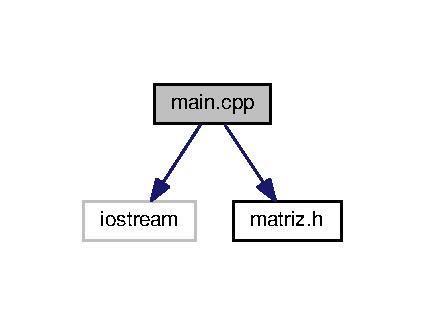
\includegraphics[width=204pt]{main_8cpp__incl}
\end{center}
\end{figure}
\subsection*{Functions}
\begin{DoxyCompactItemize}
\item 
int \hyperlink{main_8cpp_ae66f6b31b5ad750f1fe042a706a4e3d4}{main} ()
\end{DoxyCompactItemize}


\subsection{Function Documentation}
\mbox{\Hypertarget{main_8cpp_ae66f6b31b5ad750f1fe042a706a4e3d4}\label{main_8cpp_ae66f6b31b5ad750f1fe042a706a4e3d4}} 
\index{main.\+cpp@{main.\+cpp}!main@{main}}
\index{main@{main}!main.\+cpp@{main.\+cpp}}
\subsubsection{\texorpdfstring{main()}{main()}}
{\footnotesize\ttfamily int main (\begin{DoxyParamCaption}{ }\end{DoxyParamCaption})}


\hypertarget{matriz_8cpp}{}\section{matriz.\+cpp File Reference}
\label{matriz_8cpp}\index{matriz.\+cpp@{matriz.\+cpp}}
{\ttfamily \#include \char`\"{}matriz.\+h\char`\"{}}\newline
{\ttfamily \#include $<$iostream$>$}\newline
{\ttfamily \#include $<$cstdlib$>$}\newline
{\ttfamily \#include $<$cstring$>$}\newline
Include dependency graph for matriz.\+cpp\+:
\nopagebreak
\begin{figure}[H]
\begin{center}
\leavevmode
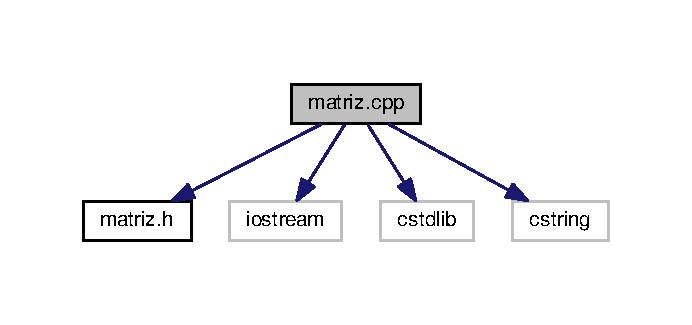
\includegraphics[width=332pt]{matriz_8cpp__incl}
\end{center}
\end{figure}

\hypertarget{matriz_8h}{}\section{matriz.\+h File Reference}
\label{matriz_8h}\index{matriz.\+h@{matriz.\+h}}
\subsection*{Classes}
\begin{DoxyCompactItemize}
\item 
class \hyperlink{class_matriz}{Matriz}
\begin{DoxyCompactList}\small\item\em The \hyperlink{class_matriz}{Matriz} class serve para realizar operacoes matematicas entre matrizes de dados do tipo float. \end{DoxyCompactList}\end{DoxyCompactItemize}

%--- End generated contents ---

% Index
\backmatter
\newpage
\phantomsection
\clearemptydoublepage
\addcontentsline{toc}{chapter}{Index}
\printindex

\end{document}
